\chapter{Manufacturing with ABS and Pumice}
\renewcommand{\baselinestretch}{\mystretch}
\label{chap:Pumice}
%\setlength{\parindent}{0pt}

\section{Methodology}
\subsection{Pumice powder}
In this project, the central issue is to demonstrate that the Martian and Lunar Regolith could be utilised for FDM technique as a raw material. As revealed by Figure \ref{Fig:mars and pumice}(a), there are some particles with the diameter large than 0.1mm among martian regolith. Similarly, the particles of Lunar regolith in Figure \ref{Fig:lunar} are also not very uniform. In order to produce a printable filament for Ultimaker 2, it is required to sieve these kinds of regolith to remain the small particles of which the diameter is less than 100$\mu$m. In fact, the basic pumice powder (599907, Pumice Powder 6/0, very fine, Kremer Pigments) in  Figure \ref{Fig:mars and pumice}(b) has the size of 0 - 90$\mu$m which is exactly suitable. Pumice is a type of volcanic rock which makes up of highly vesicular rough textured volcanic glass. Based on the SEM pictures, this kind of pumice powder could be regarded as the substitution of the Lunar and Mars dust in the experiment.  
\begin{figure}[htbp] % make the image in the middle of paragraph
	\centering
	\subfigure[]{
    \begin{minipage}[t]{0.47\textwidth}
			\centering
			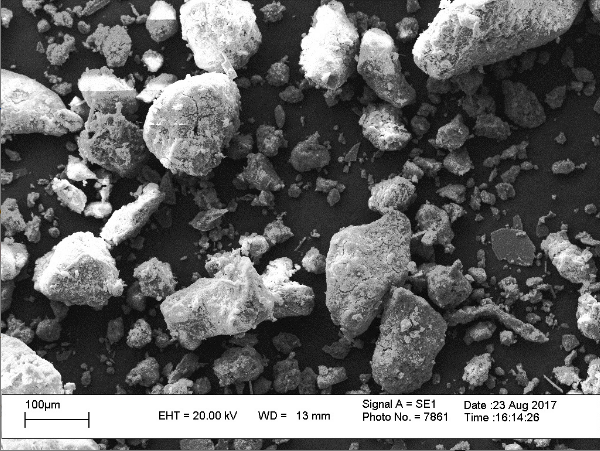
\includegraphics[height=5.5cm]{Figs4//mars_regolith.PNG}
		\end{minipage}
	}
	\subfigure[]{
		\begin{minipage}[t]{0.47\textwidth}
			\centering
			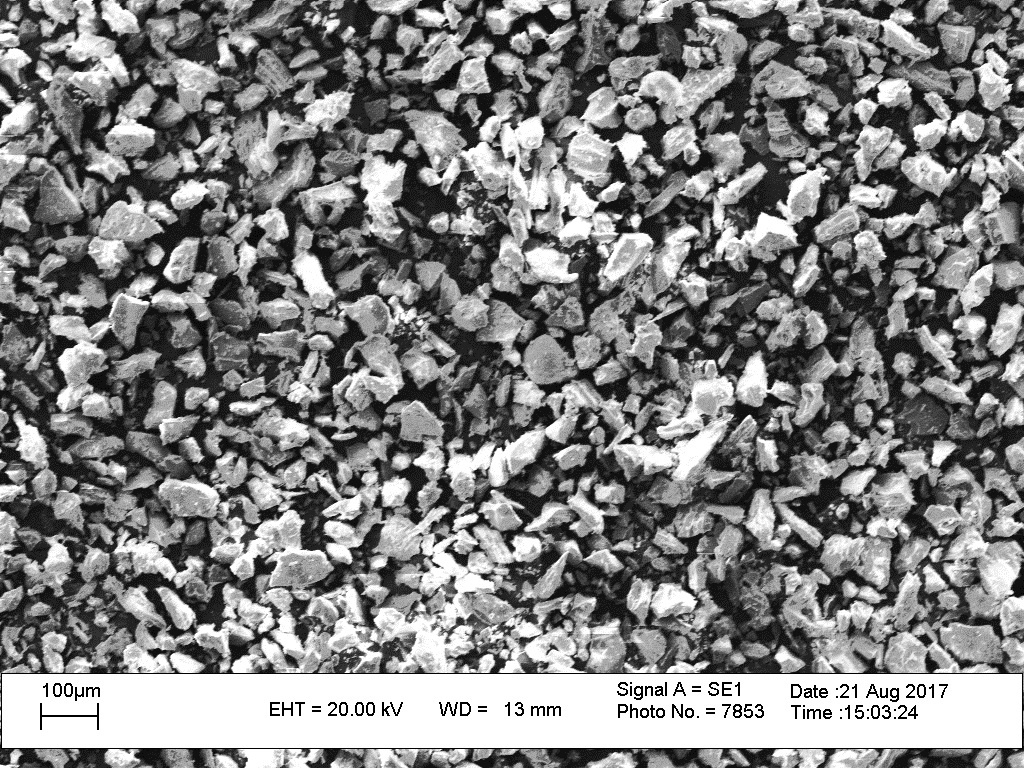
\includegraphics[height=5.5cm]{Figs4//pumice.jpg}
		\end{minipage}
	}
  \caption[SEM pictures of martian regolith and pumice powder]{\footnotesize SEM pictures of(a)martian regolith,(b) pumice powder.}
  \label{Fig:mars and pumice}
\end{figure}
\begin{figure}[htbp] % make the image in the middle of paragraph
	\centering
	\subfigure[]{
    \begin{minipage}[t]{0.47\textwidth}
			\centering
			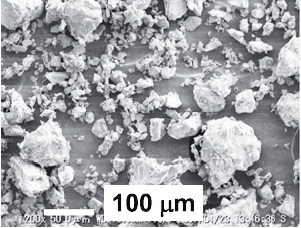
\includegraphics[height=5.5cm]{Figs4//fsd.PNG}
		\end{minipage}
	}
	\subfigure[]{
		\begin{minipage}[t]{0.47\textwidth}
			\centering
			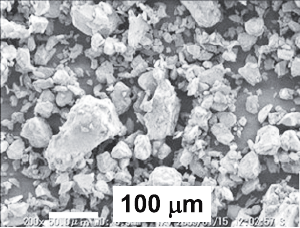
\includegraphics[height=5.5cm]{Figs4//JSC.PNG}
		\end{minipage}
	}

  \caption[SEM pictures of lunar regolith]{\footnotesize Lunar regolith simulants (a)FJS-1 ,(b)JSC-1. @copyright 2014 American Society of Civil Engineers.}
  \label{Fig:lunar}
\end{figure}
\subsection{Mixture of ABS and pumice}
Since the size and density of ABS pellets are very different from the pumice powder, it is not reasonable to directly pour them into the hopper of the extruder for the uniform filament. Ideally, powdering the ABS pellets into the same size of pumice powder could give the very uniform production. The methods to grind ABS pellets are very limited with the available facilities in our lab. And it is impossible to produce a ABS powder as fine as the pumice according to the elastic property of ABS. It is tricky that ABS material would be softened or even melted by the high power machine. The first method is to collect the small pieces of ABS by push 3mm ABS filament into a rotary tool/milling machine cutter. Another idea is using a mill coffee grinder to powdered the ABS pellets.\\
\\ 
Based on the powdered ABS and pumice, it is possible to produce the filament with different proportion of pumice and compare the weakness and advantages of specific samples. As for 3D-printability, the best way before printing is to check the consistency and smoothness of filament. 

\section{Experiment}

\subsection{Mixture of ABS and pumice with a funnel}
Firstly, the simple idea is that dropping the specific amount of ABS pellets and pumice powder into the screw with a controlled speed. The mixing work is in the dual-screw. It is not reliable to pour ABS pellets and pumice powder directly to hopper as the small particles always drop to the bottom. Based on the user's handbook of Noztek Pro Extruder, the extruding process with uniform raw materials has a relatively stable speed that we can calculate. The method was pouring a certain quantity of ABS pellets in the hopper and recording how long it takes to extrude all materials. The extrusion speed of ABS pellets at 195$^{\circ}$C in average is 0.1497g/sec. The challenge is the control of pumice powder dropping speed in order to control the amount of pumice in the filament. In this way, a funnel was designed(Figure \ref{Fig:funnel}) for guiding pumice powder. The installation of the funnel is revealed as Figure \ref{Fig:funnel install}.\\
\begin{figure}[htbp] % make the image in the middle of paragraph
	\centering
	\subfigure[]{
    \begin{minipage}[t]{1\textwidth}
			\centering
			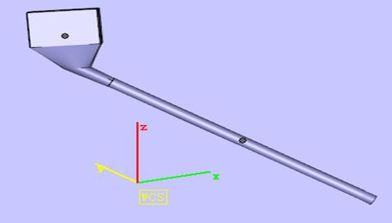
\includegraphics[width=9cm]{Figs5//funnel1.JPG}
		\end{minipage}
	}
	\subfigure[]{
		\begin{minipage}[t]{1\textwidth}
			\centering
			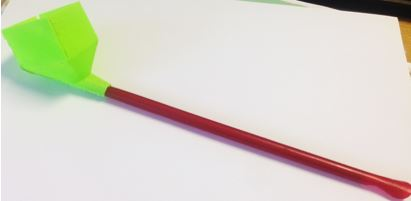
\includegraphics[width=9cm,height=5cm]{Figs5//funnel2.JPG}
		\end{minipage}
	} 
  \caption[The designed funnel]{\footnotesize (a)CAD profile of the funnel,(b)printed funnel with a screw.}
  \label{Fig:funnel}
\end{figure}
\\
After several adjusts, the pumice could drop into the hopper with a stable speed. However, the filament we got in this way is not uniform which can be seen in Figure \ref{Fig:fail}. This experiment failed since the ABS pellets covered the hole in the hopper to screw at first. The pumice powder and the ABS pellets cannot drop into the screw at the same time. The limitation of our equipment appeared in this test. Our extruder and its hopper were placed with 45 $^{\circ}$ angle to the horizontal plane. And one hopper extruder is not suitable for two different size particles extrusion together. It does not mean this method is not useful. There is a possibility that a dual-hopper extruder placed horizontally could produce homogeneous filament.

\begin{figure}[htbp] % make the image in the middle of paragraph
	\centering
	\subfigure[]{
    \begin{minipage}[t]{0.45\textwidth}
			\centering
			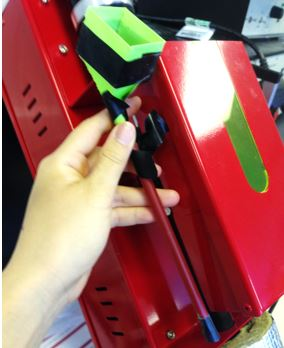
\includegraphics[height=8cm]{Figs5//funnel3.JPG}
		\end{minipage}
	}
	\subfigure[]{
		\begin{minipage}[t]{0.45\textwidth}
			\centering
			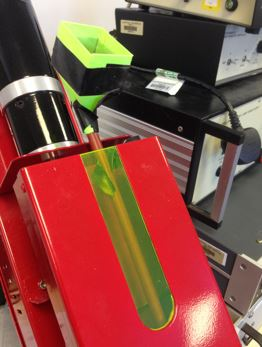
\includegraphics[height=8cm]{Figs5//funnel4.JPG}
		\end{minipage}
	} 
  \caption[The installation of the funnel]{\footnotesize The installation of the funnel.}
  \label{Fig:funnel install}
\end{figure}
\begin{figure}[htbp]
  \centering
  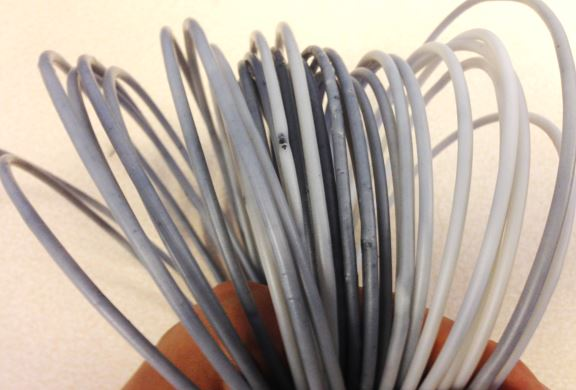
\includegraphics[scale=0.65]{Figs5//fail.JPG}
  \caption[The filament produced by the extruder and the funnel]{\footnotesize The filament produced by the extruder and the funnel.}
  \label{Fig:fail}
\end{figure}

\subsection{Mixture of ABS and pumice with a cutter}
The second method to powder ABS is using a manually-controlled cutter. The filament in Figure \ref{Fig:cutter} is with a diameter between 3.34-3.52 mm which is manufactured at 160 $^{\circ}$C. With the cutter in Figure \ref{Fig:cutter}(b), the ABS filament was powdered as \ref{Fig:cutter}(c).There are some big particles left. Compared with the size of pumice powder, this method risks the fabrication of uniform filament. After sieving these larger particles, we combined 38g powdered ABS with 2g (5 wt.$\%$) pumice powder, then used 195$^{\circ}$C as extruding temperature to obtain the filament which is very brittle and coarse\ref{Fig:filament}. Meanwhile, the powdered ABS easily absorbed moisture from the air which resulted in air bubbles in the filament.  

\begin{figure}[htbp] % make the image in the middle of paragraph
	\centering
	\subfigure[]{
    \begin{minipage}[t]{0.31\textwidth}
			\centering
			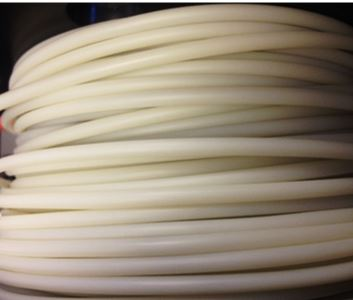
\includegraphics[height=4.2cm]{Figs4//big_filament.png}
		\end{minipage}
	}
	\subfigure[]{
		\begin{minipage}[t]{0.27\textwidth}
			\centering
			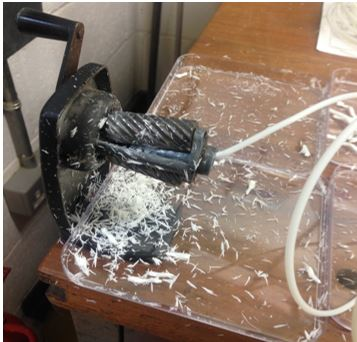
\includegraphics[height=4.2cm]{Figs4//cutter.jpg}
		\end{minipage}
	} 
 \subfigure[]{
		\begin{minipage}[t]{0.27\textwidth}
			\centering
			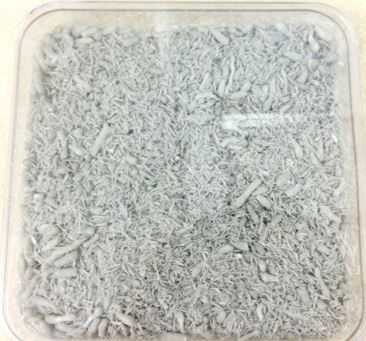
\includegraphics[height=4.2cm]{Figs4//cuttered_ABS.png}
		\end{minipage}
	}
  \caption[ABS pieces and the cutter]{\footnotesize (a)ABS filament,(b)the cutter,(c)powdered ABS .}
  \label{Fig:cutter}
\end{figure}

\begin{figure}[htbp] % make the image in the middle of paragraph
	\centering
	\subfigure[]{
    \begin{minipage}[t]{0.37\textwidth}
			\centering
			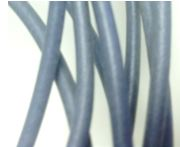
\includegraphics[height=4.5cm]{Figs4//filament.JPG}
		\end{minipage}
	}
	\subfigure[]{
		\begin{minipage}[t]{0.37\textwidth}
			\centering
			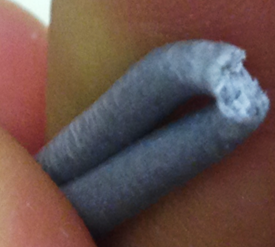
\includegraphics[height=4.5cm]{Figs4//filament_2.png}
		\end{minipage}
	}

  \caption[The quality of the filament]{\footnotesize  (a)coarse texture, (b)brittleness. }
  \label{Fig:filament}
\end{figure}

\subsection{Mixture of ABS and pumice with a coffee grinder}
Initially, the idea was use the coffee grinder (E5601BK, LLOYTRON, 150W) in Figure \ref{Fig:grinder}(a) to powder the ABS pellets. Unfortunately, it was really low-efficient work with this grinder and ABS pellets always be melted before it becomes small particles. Another problem that we cannot deal with is the moisture absorption during this process.\\
\\
After several tryings, the way to combine ABS and pumice could be worked for both the coffee grinder and the screw of extruder. The reason why we cannot pour the pumice powder and ABS pellets directly into the hopper of extruder is that the pumice powder always drops into the duality screw faster than ABS pellets. The main combination work of these two materials should be in the screw. In this view, the task of material preparation is to ensure the stable quantity of ABS and pumice drop into the screw/drill of the extruder at the same time. \\
\\
The pumice powder seems to be easily attached to slightly melted ABS pellets. The coffee grinder is used to implement this procedure creatively. The procedure as can be seen in Figure \ref{Fig:grinder}(b) and (c) is using the coffee grinder to mix ABS pellets and pumice together. This method is time efficient while the limitation obviously appeared is that the ABS cannot attach too much pumice. Moreover, the grinder will produce some ABS powder (Figure\ref{Fig:powder} after a long time grinding. In this way, there are several blends made by ABS pellets and 1 to 8 wt.$\%$ pumice are obtained. \\

\begin{figure}[htbp] % make the image in the middle of paragraph
	\centering
	\subfigure[]{
    \begin{minipage}[t]{0.25\textwidth}
			\centering
			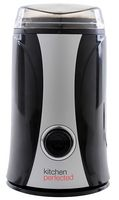
\includegraphics[height=5cm]{Figs4//grinder.jpg}
		\end{minipage}
	}
	\subfigure[]{
		\begin{minipage}[t]{0.27\textwidth}
			\centering
			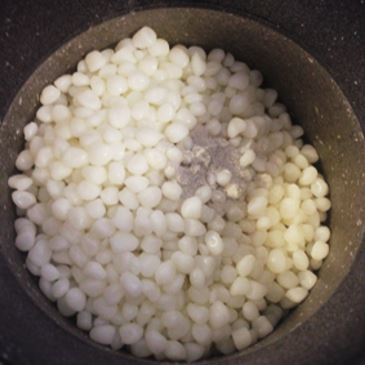
\includegraphics[height=5cm]{Figs4//abspumice1.JPG}
		\end{minipage}
	} 
 \subfigure[]{
		\begin{minipage}[t]{0.27\textwidth}
			\centering
			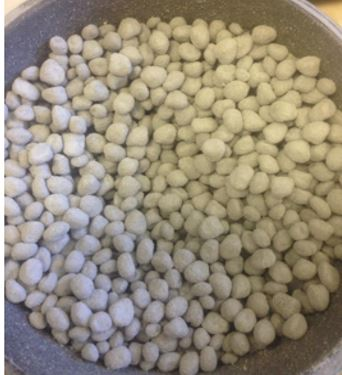
\includegraphics[height=5cm]{Figs4//abspumice2.JPG}
		\end{minipage}
	}
  \caption{Coffee grinder and the blends of ABS and pumice}{\footnotesize (a)Coffee grinder,(b)ABS and pumice,(c)blends of ABS and pumice.}
  \label{Fig:grinder}
\end{figure}

\begin{figure}[htbp] % make the image in the middle of paragraph
	\centering
	\subfigure[]{
    \begin{minipage}[t]{0.4\textwidth}
			\centering
			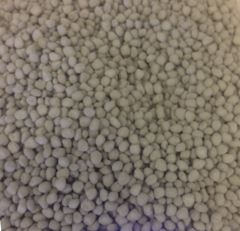
\includegraphics[height=6cm]{Figs4//abspumice3.JPG}
		\end{minipage}
	}
	\subfigure[]{
		\begin{minipage}[t]{0.4\textwidth}
			\centering
			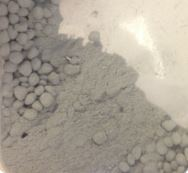
\includegraphics[height=6cm]{Figs4//powder.JPG}
		\end{minipage}
	} 

  \caption{ABS pellets and pumice powder}{\footnotesize  (a)ABS pellets with 8 wt.$\%$ pumice, (b)blends of ABS powder and pumice powder.}
  \label{Fig:powder}
\end{figure}

\subsection{Filament manufacturing}

In fact, it is significant to manufacture the 3D-printable filament with pumice powder at this stage. The key point for good printing is to make the diameter tolerance of the filament as small as possible.  Ideally, our filament should maintain an absolutely constant diameter as 2.85mm across the entire spool. However, due to small imperfections and our unprofessional extruder in the manufacturing process, there is always a tolerance of the filament diameter. In industry, the diameter tolerance could be as small as 0.05mm. It is obvious that the tolerance of our filament would be bigger than 0.05mm.\\
\\
Similar to the pure ABS filament production, the extrusion parameters could be adjusted according to the performance of products, especially the size of the filament. The performance of the filament and corresponded parameters are explained in Table \ref{tab:filament}. The mainly extruded materials are ABS pellets so that the extruding temperature could be the same as that of pure ABS. The most interesting thing is the filament shrinks when adding more than 6 wt.$\%$ pumice powder. The filament is fairly uniform as Figure \ref{Fig:FILAMENTS} shows with the exception of filament composited of ABS and 8 wt.$\%$ pumice. It is obvious that there are some blotches on the 8 wt.$\%$ pumice filament which suggests the distribution of pumice powder is not uniform. It exposes the limitation of this method that We can only make the good mixture with 7 wt.$\%$ pumice at most.\\

\begin{table}[htbp]
\centering
\caption{Extrusion parameters for filament production}
\begin{tabular}{c c c c}
\hline
\textbf{Temperature} & \textbf{Material} & \textbf{Horizontal Length} & \textbf{Filament Diameter}\\
\hline
195$^{\circ}$C & ABS with 1 wt.$\%$ pumice & 60cm & 2.78-2.98mm \\
195$^{\circ}$C & ABS with 2 wt.$\%$ pumice & 60cm & 2.85-3.05mm \\
195$^{\circ}$C & ABS with 3 wt.$\%$ pumice & 60cm & 2.83-3.03mm \\
195$^{\circ}$C & ABS with 4 wt.$\%$ pumice & 60cm & 2.84-3.02mm \\
195$^{\circ}$C & ABS with 5 wt.$\%$ pumice & 55cm & 2.84-2.97mm \\
195$^{\circ}$C & ABS with 6 wt.$\%$ pumice & 55cm & 2.80-2.92mm \\
195$^{\circ}$C & ABS with 7 wt.$\%$ pumice & 55cm & 2.77-2.88mm \\
195$^{\circ}$C & ABS with 8 wt.$\%$ pumice & 50cm & 2.65-2.75mm \\
\hline
\end{tabular}
\label{tab:filament}
\end{table}
\begin{figure}[htbp] % make the image in the middle of paragraph
	\centering
	\subfigure[]{
    \begin{minipage}[t]{0.4\textwidth}
			\centering
			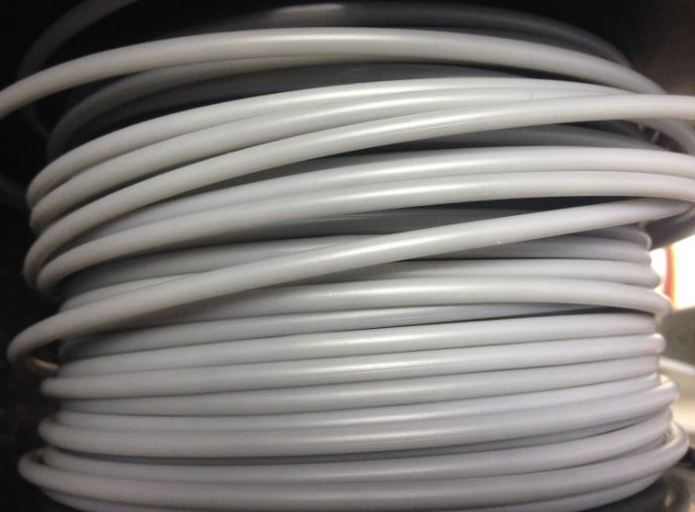
\includegraphics[height=4cm]{Figs4//3_pumice.JPG}
		\end{minipage}
	}
	\subfigure[]{
		\begin{minipage}[t]{0.4\textwidth}
			\centering
			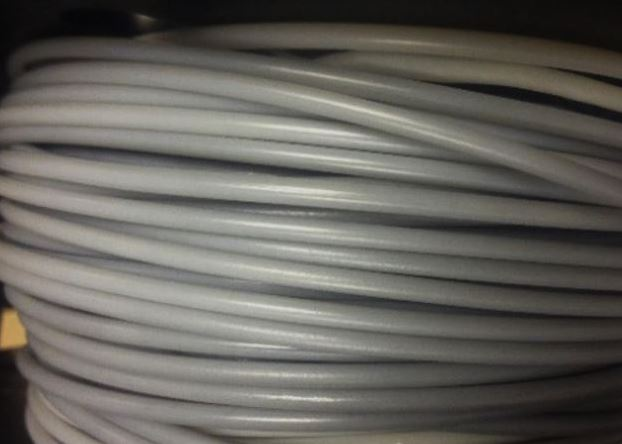
\includegraphics[height=4cm]{Figs4//5_pumice.JPG}
		\end{minipage}
	} 
    \subfigure[]{
		\begin{minipage}[t]{0.4\textwidth}
			\centering
			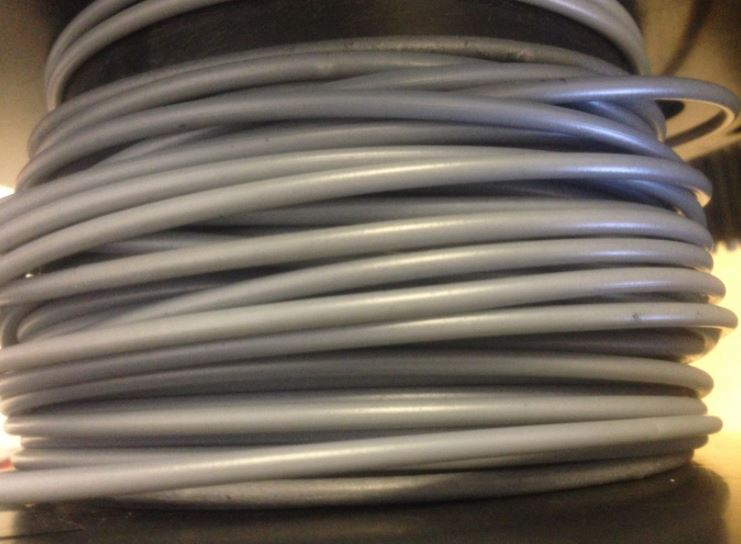
\includegraphics[height=4cm]{Figs4//7_pumice.JPG}
		\end{minipage}
	}
 \subfigure[]{
		\begin{minipage}[t]{0.4\textwidth}
			\centering
			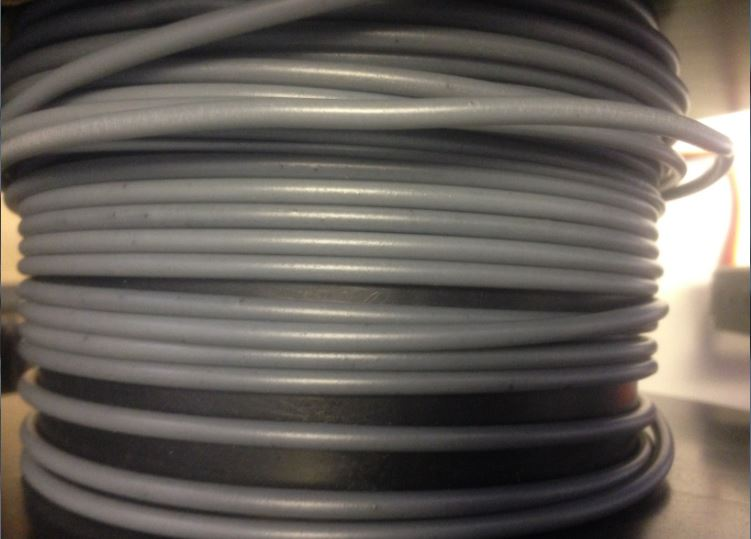
\includegraphics[height=4cm]{Figs4//8_pumice.JPG}
		\end{minipage}
	}
  \caption{The filament samples made of pumice and ABS}{\footnotesize (a)ABS with 3 wt.$\%$ pumice,  (b) ABS with 5 wt.$\%$ pumice, (c) ABS with 7 wt.$\%$ pumice, (d) ABS with 8 wt.$\%$ pumice. }
  \label{Fig:FILAMENTS}
\end{figure}

\section{Analysis}
\subsection{Meaning of adding pumice to filament}
As mentioned in chapter two, this new ink could substitute the traditional material for the space construction. From the data sheet of ABS pellets and pumice, the density of ABS pellets is 1.03 $g/cm^3$ while the density of pumice powder is 2.35 $g/cm^3$. The weight percentage could be easily transformed to voltage percentage as Table \ref{tab:ABS pumice} shows. It is highly certain that the regolith utilisation (In-situ resource utilization ) for 3D printing decreases launch and deep space transit mass and volume requirements. And it seems that this new material production contributes more to the mass saving rather than the volume saving for a space mission.  \\
\begin{table}[htbp]
\centering
\caption{The weight percentage of pumice and corresponding volume percentage}
\begin{tabular}{c  c  c}
\hline
\textbf{Weight percentage} & \textbf{Volume percentage }& \textbf{Density of the blends}\\
\hline
ABS with 0 wt.$\%$ pumice &  ABS with 0.000 vt.$\%$ pumice  &  1.030$g/cm^3$  \\
ABS with 1 wt.$\%$ pumice &  ABS with 0.441 vt.$\%$ pumice  &  1.036$g/cm^3$  \\
ABS with 2 wt.$\%$ pumice &  ABS with 0.887 vt.$\%$ pumice  &  1.041$g/cm^3$  \\
ABS with 3 wt.$\%$ pumice &  ABS with 1.337 vt.$\%$ pumice  &  1.048$g/cm^3$  \\
ABS with 4 wt.$\%$ pumice &  ABS with 1.793 vt.$\%$ pumice  &  1.054$g/cm^3$  \\
ABS with 5 wt.$\%$ pumice &  ABS with 2.255 vt.$\%$ pumice  &  1.060$g/cm^3$  \\
ABS with 6 wt.$\%$ pumice &  ABS with 2.722 vt.$\%$ pumice  &  1.066$g/cm^3$  \\
ABS with 7 wt.$\%$ pumice &  ABS with 3.194 vt.$\%$ pumice  &  1.072$g/cm^3$  \\
ABS with 8 wt.$\%$ pumice &  ABS with 3.671 vt.$\%$ pumice   & 1.078$g/cm^3$ \\
\hline
\end{tabular}
\label{tab:ABS pumice}
\end{table}

\subsection{3D-Printability of pumice filament}
From Table \ref{tab:filament}, it shows the diameter tolerance varies from 0.05mm to 0.10mm since the condition of our equipment was not stable with the same settings. The poor tolerance means that there may be some trouble when we use it in 3D printer.\\
\\
Different problems can be brought by the inhomogeneous filament diameter. A typical case is the extruder failure, a condition where the extrusion fails that no plastic is pushed down to the hot end. This might appear when your filament suddenly shrinks too much for the printer tensioning system and the mechanism offers insufficient pressure to push the filament. The too thin part of the filament will also cause back-flow and over- heating of the material in the hot end since it does not come out with the controlled flow rate. As for the too big filament diameter, there is too much material than the printer supposes it to be in the nozzle head which may block the nozzle head and cause back-flow of the material. Another influence of an increase of filament diameter is that the feeder could grind the surface of the filament and the filament stops moving to the extruder.\\
\\
After all the analysis, the diameter tolerance plays a significant role in its printable ability. Reseaching all extrusion lines in the factory, it’s very hard to go lower 0.05 mm which is already the gold standard. Since our printer was facilitated with an adjustable tensioner and the elastic stepper, it can work well with the filament which has a reasonable diameter tolerance. As we also purchased some filament from industry, we measured the diameter at several places with a calliper. The tolerance of it is 0.10mm which meets the advertised tolerance.\\
\\

\begin{figure}[htbp] % make the image in the middle of paragraph
	\centering
	\subfigure[]{
    \begin{minipage}[t]{1\textwidth}
			\centering
			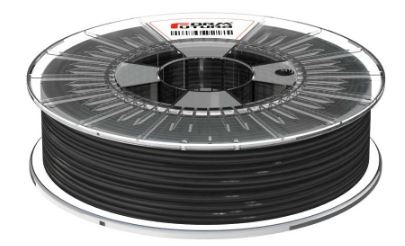
\includegraphics[height=5cm]{Figs4//ABS_easyfil.JPG}
		\end{minipage}
	}
	\subfigure[]{
		\begin{minipage}[t]{1\textwidth}
			\centering
			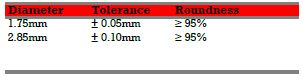
\includegraphics[height=2.5cm]{Figs4//tolerance.JPG}
		\end{minipage}
        }
  \caption{The filament purchased from Formfutura Co.}{\footnotesize  (a)The filament, (b)the diameter tolerance. }
  \label{Fig:filament}
\end{figure}


